\section{Cross-granularity prediction}
\label{app:granularity-transfer}

\paragraph{Representation states.}
The final MOSTA model specified in Section~\ref{sec:experiments} supplies native 256-dimensional molecular states without standardization. Data use follows Table~\ref{tab:evaluation_protocol}.

\paragraph{Same-location state prediction.}
For every position in each section, define $m_i^T=d^{-1}\|T_{a\to b}(e_{i,a})-e_{i,b}\|_2^2$ and $m_i^0=d^{-1}\|e_{i,a}-e_{i,b}\|_2^2$. Figure~\ref{fig:granularity-transfer}A reports $\rho_{ab}=\sum_i m_i^T/\sum_i m_i^0$ for each section. The unchanged source is the no-transformation reference; the target is directly encoded from the actual broader neighborhood at the same location. Improved-position fractions use $n^{-1}\sum_i\mathbf 1[m_i^T<m_i^0]$. Scores are computed over all positions in each evaluated section. This evaluation differs from training, where all centers within each coarse support contribute sources.

\paragraph{Projected joint association.}
Each section supplies the same fixed 2,048 positions, partitioned into four disjoint batches of 512. For each batch, correct predicted pairings, unchanged-source controls, and 20 shuffled predictions are compared with directly encoded fine--coarse pairs. Each shuffle has no fixed points and permutes only predicted destinations, preserving their marginal distribution. The product kernel uses source and target bandwidths from the corresponding observed states, shared across controls, with the settings in Appendix~\ref{app:hyperparameters}.

We evaluate the checkpoint's training projection and eight fixed orthogonal projections with seeds 2026091501--2026091508. Figure~\ref{fig:granularity-transfer}B divides the mean correct-pair MMD by the mean shuffled MMD after averaging batches and the eight fresh projections within each section. Correct pairing improves on shuffling in all 864 batch--projection--direction conditions. Compared with the unchanged source on the training projection, transformation lowers joint discrepancy in 21 of 24 section--direction conditions. All three exceptions are in E12.5 E2S1; its projected joint discrepancy increases for each training direction. Table~\ref{tab:granularity-transfer-sections} reports every section and direction.

\begin{figure}[!htbp]
\centering
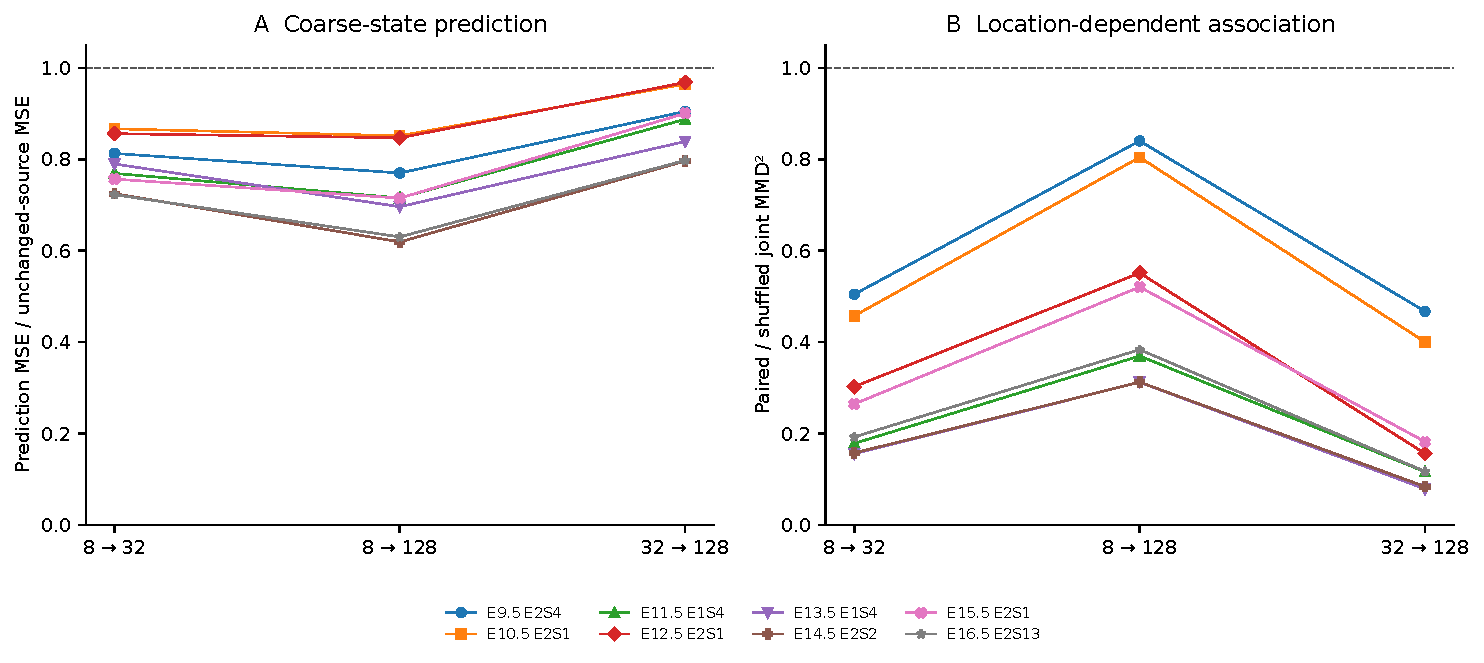
\includegraphics[width=\linewidth]{figures/granularity_transfer.pdf}
\caption{\textbf{Predictive relationships across held-out tissue sections.} \textbf{A}, Target-MSE ratio of transformed to untransformed fine states, using the same directly encoded coarse reference. \textbf{B}, Joint-MMD ratio of correct to shuffled predicted pairings, averaged over four batches and eight projections unused in training. Each line denotes one section; values below one favor the learned prediction or correct pairing.}
\label{fig:granularity-transfer}
\end{figure}

\begin{table}[!htbp]
\centering\small
\caption{\textbf{Coarse-state prediction on every held-out section.} MSE ratio compares transformed and unchanged sources against the same encoded coarse target. Improved is the percentage of positions with lower MSE. Paired/shuffled is the joint-MMD ratio averaged over batches and fresh projections.}
\label{tab:granularity-transfer-sections}
\begin{tabular}{lcccc}
\toprule
Section & Pair & MSE ratio & Improved (\%) & Paired/shuffled \\
\midrule
E9.5 E2S4 & 8$\to$32 & 0.813 & 98.0 & 0.505 \\
E9.5 E2S4 & 32$\to$128 & 0.905 & 84.3 & 0.467 \\
E9.5 E2S4 & 8$\to$128 & 0.770 & 98.3 & 0.840 \\
E10.5 E2S1 & 8$\to$32 & 0.867 & 88.7 & 0.458 \\
E10.5 E2S1 & 32$\to$128 & 0.965 & 58.7 & 0.400 \\
E10.5 E2S1 & 8$\to$128 & 0.851 & 88.7 & 0.804 \\
E11.5 E1S4 & 8$\to$32 & 0.769 & 97.9 & 0.178 \\
E11.5 E1S4 & 32$\to$128 & 0.888 & 82.3 & 0.116 \\
E11.5 E1S4 & 8$\to$128 & 0.715 & 98.2 & 0.370 \\
E12.5 E2S1 & 8$\to$32 & 0.856 & 88.9 & 0.302 \\
E12.5 E2S1 & 32$\to$128 & 0.968 & 53.7 & 0.156 \\
E12.5 E2S1 & 8$\to$128 & 0.847 & 84.1 & 0.551 \\
E13.5 E1S4 & 8$\to$32 & 0.790 & 97.4 & 0.156 \\
E13.5 E1S4 & 32$\to$128 & 0.839 & 89.0 & 0.079 \\
E13.5 E1S4 & 8$\to$128 & 0.696 & 98.5 & 0.312 \\
E14.5 E2S2 & 8$\to$32 & 0.725 & 98.6 & 0.157 \\
E14.5 E2S2 & 32$\to$128 & 0.796 & 91.9 & 0.084 \\
E14.5 E2S2 & 8$\to$128 & 0.619 & 99.5 & 0.312 \\
E15.5 E2S1 & 8$\to$32 & 0.757 & 93.9 & 0.265 \\
E15.5 E2S1 & 32$\to$128 & 0.900 & 59.2 & 0.182 \\
E15.5 E2S1 & 8$\to$128 & 0.715 & 91.7 & 0.521 \\
E16.5 E2S13 & 8$\to$32 & 0.722 & 97.9 & 0.192 \\
E16.5 E2S13 & 32$\to$128 & 0.798 & 91.4 & 0.117 \\
E16.5 E2S13 & 8$\to$128 & 0.630 & 98.3 & 0.383 \\
\bottomrule
\end{tabular}

\end{table}
